% Diapositiva 21

% Kevin
%=============================================
% 2. Explicar por qué se construye una función de error
% 3. Explicar qué significa minimizar el error
% 4. Explicar por qué se usan mínimos cuadrados
% 5. Introducir la función de error
%=============================================

\begin{frame}{Construcción de la Función de Error}

    \begin{columns}[T]
        %========================================
        % COLUMNA IZQUIERDA: VISUALIZACIÓN
        %========================================
        \column{0.50\textwidth}
        \begin{center}
            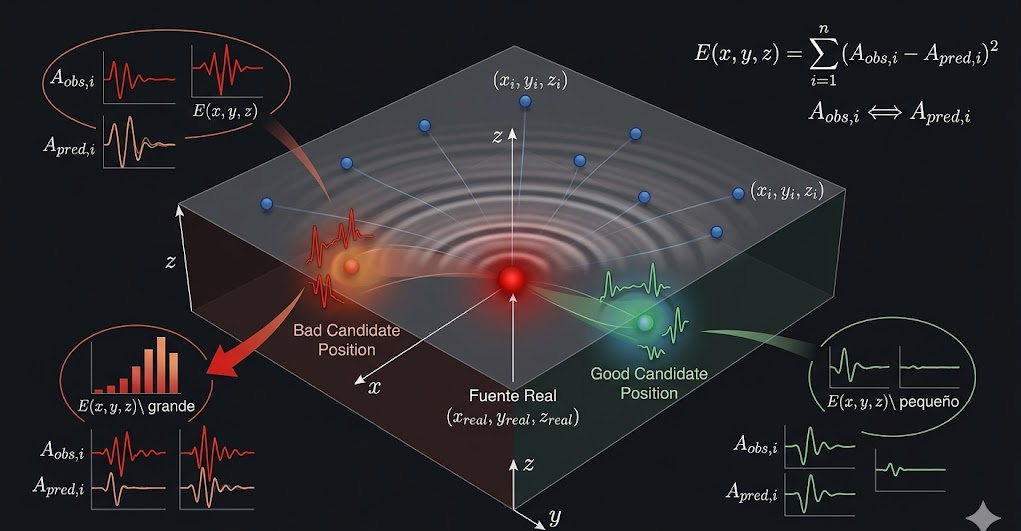
\includegraphics[width=0.95\textwidth]{Imagenes/FuncionErroryMinimizacion.png}
        \end{center}

        \vspace{-0.2cm}
        \begin{center}
            \tiny \textcolor{gray}{
            Superficie matemática del error acumulado de la red.
            }
        \end{center}

        %========================================
        % COLUMNA DERECHA: MÉTRICA Y JUSTIFICACIÓN
        %========================================
        \column{0.46\textwidth}

        \begin{block}{Métrica de Ajuste Global}
            \centering
            \small
            \[ E(x,y,z) = \sum_{i=1}^{n} \left( A_{obs,i} - A_{pred,i} \right)^2 \]
        \end{block}

        \vspace{0.1cm}

        \begin{block}{¿Por qué Mínimos Cuadrados?}
            \scriptsize
            \begin{itemize}
                \item \textbf{Sin Cancelación:} Evita que errores positivos y negativos se anulen entre sí.
                \item \textbf{Penalización:} Magnifica fuertemente las discrepancias más grandes.
            \end{itemize}
        \end{block}

        \vspace{0.1cm}

        \begin{block}{Restricción del Modelo}
            \scriptsize
            \textbf{Optimización espacial:} La amplitud inicial $A_0 = 10$ se mantiene fija. La búsqueda se realiza únicamente sobre $(x,y,z)$.
        \end{block}

    \end{columns}

    \vspace{0.3cm}
    \begin{center}
        \footnotesize 
        \textbf{La función mide qué tan distante es la respuesta teórica frente a la realidad medida.}
    \end{center}

\end{frame}